\documentclass[11pt,a4paper]{article}

% ------------------------
% Packages
% ------------------------
\usepackage[utf8]{inputenc}
\usepackage[T1]{fontenc}
\usepackage{lmodern}

\usepackage{geometry}
\geometry{margin=2.5cm}

\usepackage{setspace}
\onehalfspacing

\usepackage{graphicx}
\usepackage{amsmath, amssymb}

\usepackage{booktabs}
\usepackage{array}
\usepackage{multirow}

\usepackage{hyperref}
\hypersetup{
    colorlinks=true,
    linkcolor=black,
    citecolor=black,
    urlcolor=black
}

\usepackage{caption}
\usepackage{subcaption}

\usepackage{enumitem}
\usepackage{pgfplots}
\pgfplotsset{compat=1.18}

% Chart colours for the three configurations compared with the static pipeline
\definecolor{cleaning}{HTML}{2A78D6}
\definecolor{metaonly}{HTML}{EB6834}
\definecolor{fullsystem}{HTML}{1BAF7A}

% ------------------------
% Title Information
% ------------------------
\title{\textbf{Intelligent Automation of Data Preparation Using Meta-Learning and Performance-Driven Optimization}}

\author{
    Parinaz Teimouri \\
    Applied Computer Science \\
    FH Schmalkalden University of Applied Sciences \\
    \texttt{p.teimouri@stud.fh-sm.de}
}

\date{\today}

% ------------------------
% Document
% ------------------------
\begin{document}
\maketitle

% ---------------- ABSTRACT ----------------
\begin{abstract}
Data preparation is a critical yet time-consuming stage in machine learning workflows, often requiring extensive manual intervention and expert knowledge. Despite recent progress in automated machine learning systems, data preprocessing remains largely dependent on static heuristics and dataset-agnostic rules. This paper presents an automated, performance-driven data preparation framework for tabular data. The system repairs inconsistent values, keeps the target column out of every preprocessing step, and selects strategies for missing value imputation and feature scaling by combining a meta-learned shortlist with cross-validated downstream evaluation; categorical encoding and outlier handling follow meta-features and robust statistics. Every decision is logged, so the process stays transparent and reproducible. In a benchmark on seven datasets with five random splits each, the full system outperformed a static pipeline in 28 of 35 paired comparisons, with a mean gain of 0.018 in macro F1 or $R^2$. An ablation shows that about 90\% of this gain comes from automatic value cleaning, while performance-driven strategy selection adds only 0.002 over well-chosen fixed defaults, and meta-features of a single column do not reliably predict the best strategy. Open challenges and future research directions toward global pipeline optimization are also discussed.
\end{abstract}

\noindent\textbf{Keywords:} Automated Data Preparation, Meta-Learning, Tabular Data, Machine Learning Pipelines, Feature Engineering


% ---------------- BACKGROUND ----------------
\section{Scientific Background and Related Knowledge}

The success of machine learning models depends not only on algorithmic design but also, to a significant extent, on the quality of the input data. In practical applications, raw data frequently contains missing values, inconsistent formats, outliers, and heterogeneous feature types. Studies have shown that data preparation can account for up to 80\% of the total time spent in applied machine learning projects.

Traditional data preprocessing pipelines rely heavily on handcrafted rules, such as mean imputation for missing values or one-hot encoding for categorical variables. While effective in limited scenarios, these heuristics fail to generalize across datasets with diverse statistical properties. Furthermore, inappropriate preprocessing choices may significantly degrade downstream model performance.

Automated Machine Learning (AutoML) frameworks aim to reduce human intervention by automating model selection and hyperparameter tuning. However, many AutoML systems either assume preprocessed data or apply simplistic preprocessing strategies that are not optimized for the specific dataset. As a result, preprocessing remains a bottleneck in achieving fully autonomous machine learning systems.

Recent research has explored meta-learning approaches to address this limitation. Meta-learning leverages knowledge from prior datasets to guide decision-making on new datasets by learning relationships between dataset characteristics and optimal strategies. While promising, existing approaches often focus on individual preprocessing steps and lack empirical validation using downstream performance metrics.

This work builds upon these ideas by treating data preparation as a performance-driven optimization problem, in which preprocessing strategies are selected based on both dataset meta-features and their measurable impact on predictive performance.


\subsection{Limitations of Rule-Based Data Preparation}

Rule-based data preparation pipelines remain the dominant approach in practical machine learning systems. These pipelines typically rely on fixed thresholds and generic assumptions, such as imputing missing values using the mean or encoding all categorical variables using one-hot encoding. While such approaches are computationally efficient, they implicitly assume that all datasets share similar statistical characteristics, which is rarely the case in real-world scenarios.

One major limitation of static preprocessing rules is their inability to adapt to dataset-specific distributions. For example, mean imputation may introduce significant bias when applied to skewed data, while one-hot encoding can lead to dimensionality explosion in high-cardinality categorical features. Moreover, these preprocessing choices are often made independently, ignoring interactions between steps such as imputation and scaling.

Another critical issue is the lack of objective evaluation criteria for preprocessing quality. In many cases, preprocessing decisions are justified heuristically rather than empirically, leading to pipelines that are suboptimal for the target task. This motivates the need for adaptive and performance-aware preprocessing systems that can evaluate the impact of each transformation on downstream model performance.

\subsection{Data Preparation as an Optimization Problem}

From a formal perspective, data preparation can be modeled as an optimization problem. Let $D$ denote the raw dataset and $\mathcal{P}$ the space of all possible preprocessing pipelines. Each pipeline $p \in \mathcal{P}$ transforms $D$ into a processed dataset $D_p$, which is subsequently used to train a machine learning model $M$.

The objective is to select the pipeline $p^*$ that maximizes a performance metric $J$, such that:

\[
p^* = \arg\max_{p \in \mathcal{P}} J(M(D_p))
\]

However, the pipeline space $\mathcal{P}$ grows exponentially with the number of preprocessing steps and candidate strategies, rendering exhaustive search infeasible. As a result, practical systems must rely on heuristics, approximations, or local optimization strategies. The proposed framework adopts a modular and greedy optimization approach, selecting locally optimal strategies at each preprocessing stage based on empirical evaluation.


% ---------------- OPEN TOPIC ----------------
\section{Selected Open Topic}

The selected open research topic of this paper is the development of a fully automated and adaptive data preparation system for tabular machine learning. Specifically, the focus lies on addressing the following open challenges:

\begin{itemize}
    \item How can preprocessing strategies be selected dynamically instead of relying on static heuristics?
    \item How can preprocessing quality be evaluated objectively?
    \item How can automation be achieved without sacrificing transparency and reproducibility?
\end{itemize}

This topic remains open due to the inherent complexity of preprocessing decisions and the exponential search space of possible preprocessing pipelines. Rather than aiming for global optimization, this work investigates a locally optimal, modular approach that balances performance, interpretability, and computational efficiency.

% ---------------- METHODS ----------------
\section{Methods}

\subsection{System Architecture}

The proposed framework is implemented as a modular Python pipeline centered around the \texttt{AutoDataPreparer} class, with the meta-learning component in a separate module. Each preprocessing task is encapsulated in its own step, allowing flexible extension and clear separation of concerns. The pipeline runs the following stages in order:

\begin{enumerate}[noitemsep]
    \item \textbf{Load:} CSV files in any common encoding and delimiter (including German Excel exports separated by semicolons), or Excel files.
    \item \textbf{Target separation:} the column to predict is set aside.
    \item \textbf{Value standardisation:} yes/no text, numbers stored as text and spelling variants are repaired.
    \item \textbf{Task type detection:} classification or regression.
    \item \textbf{Date parsing:} date columns are decomposed into year, month and day.
    \item \textbf{Deduplication:} exact duplicate rows are removed.
    \item \textbf{Identifier exclusion:} ID and free-text columns are left out of the features.
    \item \textbf{Outlier treatment:} rare extremes are capped.
    \item \textbf{Missing value imputation.}
    \item \textbf{Categorical encoding.}
    \item \textbf{Feature scaling.}
\end{enumerate}

Two files are produced. The \emph{human-readable} output is taken after imputation: it contains the identifiers, the repaired values and the original (uncapped) values, so that every row can be traced. The \emph{ML-ready} output is encoded and scaled. Standardisation runs before deduplication so that rows differing only in spelling (``Male'' and ``male'') are recognised as duplicates.

\subsection{Target Separation}

When a target column is given, it is removed from the features before any other step and only re-attached when the output is written. No capping, imputation or scaling can alter it, and no candidate evaluation can use it as a feature, which would otherwise leak the label into the score. Rows without a target value are dropped, since they cannot be used for supervised evaluation. The target receives the same text repairs as the features (for example, prices stored as text become numbers), but never imputation or scaling.

\subsection{Value Standardisation}

Real exports often contain the same information in inconsistent forms. Each text column is checked for three kinds of defects, and the first that applies is repaired:

\begin{itemize}
    \item \textbf{Yes/no text.} If every value belongs to a set of boolean tokens (yes/no, y/n, true/false, 1/0 and the German ja/nein, wahr/falsch), the column becomes 0/1.
    \item \textbf{Numbers stored as text.} Currency markers and percent signs are removed, and decimal commas, German thousands separators and English thousands separators are recognised (``89,90~\texteuro'', ``1.299,00'', ``EUR 1,299.00'', ``84\%''). If at least 90\% of the values can be read, the column becomes numeric and the remaining values become missing.
    \item \textbf{Spelling variants.} Values that differ only in case or whitespace are merged (``NAVY'', ``navy\textvisiblespace'', ``Navy''). In columns with at most ten categories, a single letter joins the only longer value that starts with it (``m'' $\rightarrow$ ``male''). The form used most often wins.
\end{itemize}

Columns named like identifiers are kept exactly as written: an invoice number such as ``C536379'' is not a broken number.

\subsection{Identifier Detection}

Identifier and free-text columns describe individual rows and carry no signal that generalises to new data; one-hot encoding them only inflates the feature space. A column is excluded from the ML features if it holds text with at least 95\% distinct values, or if its name marks it as an identifier (name parts such as \emph{id}, \emph{sku} or \emph{ean}, or the suffixes \emph{no} and \emph{nr}) and it has many distinct values (at least 95\% distinct, or at least $\max(20, 0.05\,n)$ for $n$ rows). A customer ID that repeats across orders is therefore still treated as a key, while a \texttt{store\_id} with five stores remains a category. Excluded columns stay in the human-readable output.

\subsection{Task Type Detection}

Before preprocessing, the system automatically determines whether the learning task is classification or regression from the repaired target. Non-numeric targets are treated as classification. Numeric targets with fractional values (such as a rating of 3.3) are treated as regression; integer-valued targets with fewer than 20 distinct values, or fewer than 5\% distinct values, are treated as classification, and all other targets as regression. This distinction allows the system to select appropriate evaluation metrics and downstream models.

\subsection{Meta-Feature Extraction}

For each preprocessing decision, a set of meta-features is extracted from one column to characterize its statistical properties (Table~\ref{tab:metafeatures}). For imputation the column with the most missing values is described, for scaling the column with the largest absolute skewness, and for encoding each categorical column individually. The meta-features serve as input to the meta-learning component responsible for narrowing down candidate preprocessing strategies.

\begin{table}[h]
\centering
\caption{Extracted Meta-Features}
\label{tab:metafeatures}
\begin{tabular}{ll}
\toprule
\textbf{Meta-Feature} & \textbf{Description} \\
\midrule
Number of Rows & Size of the dataset \\
Missing Ratio & Proportion of missing values \\
Skewness & Distribution asymmetry (0 for categorical columns) \\
Kurtosis & Distribution tail heaviness (0 for categorical columns) \\
Unique Ratio & Distinct values divided by the number of rows \\
Data Type & Numeric or categorical indicator \\
\bottomrule
\end{tabular}
\end{table}

\subsection{Missing Value Imputation}

Missing value handling is formulated as a strategy selection problem. For numerical features, the candidate strategies are mean imputation, median imputation and $k$-nearest neighbors imputation ($k=5$); the selected strategy is applied to all numerical columns. Binary 0/1 columns are filled with their most frequent value instead, since a mean of 0.67 is not a valid flag.

Categorical features with few gaps are filled with their most frequent category. Columns with more than 10\% missing values, or with more than 50 distinct values, receive an explicit \texttt{(missing)} category instead: copying the most common value (for example, one product description) into many rows would invent a pattern that is not in the data.

\subsection{Categorical Encoding}

For each categorical column, the meta-learner chooses between one-hot encoding (dropping the first level) and label encoding, based on the column's meta-features. Without a trained meta-model, a fixed rule applies: one-hot encoding if fewer than 5\% of the values are distinct, label encoding otherwise, which prevents dimensionality explosion in high-cardinality features. Encoding is predicted but, unlike imputation and scaling, not evaluated against the target. A non-numeric classification target is label-encoded separately.

\subsection{Feature Scaling}

Numerical features are scaled using a performance-driven selection mechanism. Candidate scaling strategies are standardization, min-max scaling and robust scaling; binary columns are not scaled. Because tree-based models are invariant to rescaling a feature, the scaling candidates are compared with a scale-sensitive $k$-nearest neighbors model ($k=5$) instead of a random forest.


\subsection{Outlier Detection and Treatment}

The framework implements a context-aware outlier management strategy designed to balance data integrity with statistical robustness. The process involves two distinct phases: detection and adaptive treatment.

\subsubsection{Detection Mechanism}
Initial detection is performed using robust statistical metrics rather than computationally expensive anomaly detection algorithms. Specifically, the system utilizes the Interquartile Range (IQR) method to characterize the distribution of each numerical feature. By calculating the first ($Q_1$) and third ($Q_3$) quartiles, the system identifies potential outliers that fall outside the standard boxplot whiskers defined by $1.5 \times \text{IQR}$. Constant columns ($\text{IQR} = 0$) are skipped.

\subsubsection{Adaptive Winsorization}
Once potential outliers are identified, the system calculates the outlier ratio relative to the total number of observations. The treatment strategy is then branched based on a dynamic threshold:

\begin{itemize}
    \item \textbf{Rare Outliers ($< 5\%$):} If the outlier frequency is identified as rare, the system applies IQR-based Winsorization, capping extreme values at the boundaries:
    \begin{equation}
        [Q_1 - 1.5 \times \text{IQR}, \quad Q_3 + 1.5 \times \text{IQR}]
    \end{equation}
    This approach neutralizes the influence of extreme noise while preserving the total sample size and dataset power.

    \item \textbf{Heavy-Tailed Distributions ($\geq 5\%$):} If the outlier ratio exceeds this threshold, the system characterizes the feature as naturally heavy-tailed. In such cases, original values are preserved to prevent the distortion of significant structural information that may be essential for downstream predictive performance.
\end{itemize}

Capping applies to the ML-ready output only. The human-readable output restores the original values, so that a genuinely high price is never silently changed in the file a person reads.


\subsection{Decision Transparency}

All preprocessing decisions are logged via a dedicated DecisionLogger class. This component generates a comprehensive JSON execution report that includes a \texttt{changes\_summary}, detailing every column transformation, the specific action taken (e.g., ``Winsorization'' or ``Label Encoding''), and the number of affected rows. The report also records the candidate strategies and their scores, how many rows were removed and why (duplicates, missing or unreadable target values) and the time spent in each stage. This ensures that while the process is automated, it remains fully auditable and reproducible for the end user.

\subsection{Top-K Strategy Selection}

To optimize performance while managing the exponential search space, the system utilizes a Top-K optimization strategy for imputation and scaling:
\begin{itemize}
    \item \textbf{Phase 1: Meta-learning filter.} The MetaLearner ranks all candidate strategies for the task from the extracted meta-features, and the top $k$ are kept; in the current implementation, $k$ is set to 2. Without a trained meta-model, the ranking is the fixed rule's choice followed by the remaining strategies in a fixed order. Strategies that are too expensive for the dataset are removed from the ranking (see Section~\ref{sec:complexity}).
    \item \textbf{Phase 2: Empirical evaluation.} Each candidate is plugged into a complete scikit-learn pipeline in which the other steps use safe defaults (median imputation, one-hot encoding, standardization), and the pipeline is scored with 3-fold cross-validation, stratified for classification. Imputation candidates are scored with a random forest (50 trees), scaling candidates with $k$-nearest neighbors.
    \item \textbf{Selection.} The strategy yielding the highest macro $F1$-score (for classification) or $R^2$ (for regression) is selected and applied to the dataset. If every evaluation fails, the meta-learner's top-ranked candidate is used. The winner is stored as feedback for future meta-training.
\end{itemize}

\subsection{Meta-Model Training}

The meta-learner consists of one random forest classifier (100 trees) per task that maps the six meta-features to the best strategy. Its training labels are empirical rather than hand-written. A training script generates synthetic supervised datasets with 150 to 1,499 rows and 4 to 11 features, for classification or regression with varying noise. For imputation and scaling, a random subset of columns is made skewed or heavy-tailed (exponential and quadratic transformations, injected extreme values), and for imputation, missing values are added (5--50\% per affected column). For encoding, one column is turned into 2 to 59 categories, whose names are unrelated to the underlying order in half of the cases. Each dataset is labelled with the candidate strategy that scores best under exactly the same cross-validated evaluation the pipeline uses, so the meta-model learns to predict measured outcomes. Feedback stored by real pipeline runs is added to this training data, closing the learning loop.




\subsection{Pipeline Decision Flow}

The preprocessing pipeline follows a sequential decision-making process, where each stage operates on the output of the previous one. This design reflects realistic machine learning workflows and ensures compatibility with standard modeling tools.

At each evaluated stage, a finite set of candidate strategies is defined. Rather than selecting a strategy solely based on meta-features, the system evaluates the shortlisted candidates by training a downstream model and measuring its predictive performance. This empirical evaluation acts as a proxy for preprocessing quality.

To limit computational overhead, the evaluation models are intentionally small (a random forest with 50 trees, or $k$-nearest neighbors for scaling). That relative differences between strategies carry over to the final production model is an assumption rather than a guarantee; the benchmark therefore scores the prepared data with two different downstream models.

\subsection{Computational Complexity Considerations}
\label{sec:complexity}

While performance-driven selection can improve preprocessing quality, it introduces additional computational cost. Let $k$ denote the number of candidate strategies at a preprocessing stage, $f$ the number of cross-validation folds and $n$ the number of samples. The time complexity of each evaluated stage can be approximated as:

\[
\mathcal{O}(k \cdot f \cdot T_{model}(n))
\]

where $T_{model}(n)$ denotes the training time of the evaluation model. Top-K filtering bounds $k$ at 2 instead of all candidates, and the evaluation models are kept small. In addition, strategies are pruned up front based on dataset size: $k$-nearest neighbors imputation scales quadratically with the number of rows and is excluded above 10,000 rows. In the benchmark, the full system took 0.36\,s per run on average, including strategy selection, compared with 0.17\,s for the static pipeline.

\subsection{Automated Feature Engineering and Type Enforcement}

Beyond standard preprocessing, the system implements specialized heuristics for temporal data and schema consistency. The \texttt{parse\_dates} step samples up to 100 values of each text column; if more than 80\% are shaped like dates (digit groups joined by a separator) and more than 80\% can be parsed, the column is treated as temporal. Dates written with dots (``01.12.2010'') are read day-first, as is customary in Germany. Temporal columns are decomposed into year, month and day to allow standard machine learning algorithms to capture seasonal patterns, and the original date column is dropped before encoding. Additionally, the framework records which numeric columns originally held only whole numbers (such as ages, counts or flags) and rounds them back to integers after imputation or capping has introduced fractions.


% ---------------- RESULTS ----------------
\section{Results}

\subsection{Experimental Setup}

The system was evaluated with a reproducible benchmark script on seven tabular datasets:

\begin{itemize}
    \item \textbf{Three datasets with injected defects:} the scikit-learn breast cancer and wine datasets (classification) and the diabetes dataset (regression). Defects of the kind found in real exports were added: a third of the columns were skewed, 20\% of values were removed in half of the columns and value-dependent gaps were added to one more, one column was stored as currency text in mixed formats, one informative column was replaced by a category written in four spellings, another by a yes/no flag in mixed notation, and an ID column was added.
    \item \textbf{A messy export:} a freelancer dataset from the repository (899 rows, regression on the rating), used as delivered.
    \item \textbf{Three real datasets from OpenML}, used as they are: Titanic (1,309 rows; the lifeboat and body number columns were dropped because they are recorded after the fact and reveal the target), a 3,000-row sample of the adult census data, and German credit (credit-g, 1,000 rows), all classification.
\end{itemize}

Four configurations were compared. All of them share deduplication, outlier treatment and date expansion:

\begin{itemize}
    \item \textbf{Static:} mean imputation, one-hot encoding and standardization, without value cleaning.
    \item \textbf{Static + cleaning:} the same fixed strategies, plus value standardisation and identifier exclusion.
    \item \textbf{Meta-model only:} cleaning, with strategies predicted by the meta-learner but not evaluated.
    \item \textbf{Full system:} cleaning with Top-K evaluation against the target (the proposed method).
\end{itemize}

No meta-models were trained for the main run, so the meta-learner used its fixed rules: ``meta-model only'' is rule-based prediction, and the full system evaluates the rules' two highest-ranked candidates.

Each dataset was split into a selection half and an evaluation half (stratified for classification), repeated with five different random splits. The full system chose its imputation and scaling strategies on the selection half only; these choices were then applied to the evaluation half, so no configuration was scored on rows it was tuned on. Each prepared evaluation half was scored with two downstream models, a linear model (logistic regression or ridge regression) and a random forest with 100 trees, using 5-fold cross-validation: macro F1 for classification, $R^2$ for regression. The reported score is the mean over both models. Within the evaluation half, preprocessing is fitted on all rows before cross-validation. This is identical for every configuration, so comparisons are fair, but absolute scores are slightly optimistic.

\subsection{Downstream Performance}

Table~\ref{tab:results} shows the mean score of each configuration and Figure~\ref{fig:gain} the gain over the static pipeline. The static pipeline has the worst mean rank (3.50); the three configurations with value cleaning are close together (2.07 to 2.21). The gains are concentrated on the datasets with defects: 0.017 on breast cancer, 0.030 on wine, 0.026 on diabetes and 0.043 on the freelancer export for the full system. On the three real OpenML datasets, which contain few of the defects the cleaning step repairs, all configurations lie within 0.007 of each other. On the freelancer data every configuration scores below zero, meaning that the rating is barely predictable from the other columns; cleaning still reduces the error clearly.

\begin{table}[ht]
\centering
\small
\caption{Downstream performance: macro F1 (classification) or $R^2$ (regression) on the evaluation half, averaged over a linear model and a random forest. Mean (standard deviation) over five splits; best per row in bold; $^\ast$ = injected defects.}
\label{tab:results}
\setlength{\tabcolsep}{3.5pt}
\begin{tabular}{llcccc}
\toprule
\textbf{Dataset} & \textbf{Task} & \textbf{Static} & \textbf{Static + cleaning} & \textbf{Meta-model only} & \textbf{Full system} \\
\midrule
adult & class. & \textbf{0.772} (0.015) & \textbf{0.772} (0.015) & 0.772 (0.015) & 0.772 (0.015) \\
breast cancer$^\ast$ & class. & 0.936 (0.010) & 0.950 (0.010) & 0.949 (0.007) & \textbf{0.953} (0.011) \\
credit-g & class. & 0.661 (0.013) & 0.667 (0.015) & 0.668 (0.015) & \textbf{0.668} (0.015) \\
diabetes$^\ast$ & regr. & 0.280 (0.054) & 0.304 (0.027) & \textbf{0.309} (0.036) & 0.306 (0.030) \\
freelancers & regr. & $-$0.155 (0.042) & $-$0.111 (0.023) & \textbf{$-$0.111} (0.027) & $-$0.112 (0.024) \\
titanic & class. & 0.777 (0.019) & \textbf{0.781} (0.020) & 0.779 (0.020) & 0.777 (0.017) \\
wine$^\ast$ & class. & 0.941 (0.024) & 0.961 (0.024) & 0.964 (0.015) & \textbf{0.971} (0.014) \\
\midrule
\multicolumn{2}{l}{Mean rank (1 = best)} & 3.50 & 2.21 & \textbf{2.07} & 2.21 \\
\multicolumn{2}{l}{Mean preparation time (s)} & 0.17 & 0.12 & 0.08 & 0.36 \\
\bottomrule
\end{tabular}
\end{table}

\begin{figure}[ht]
\centering
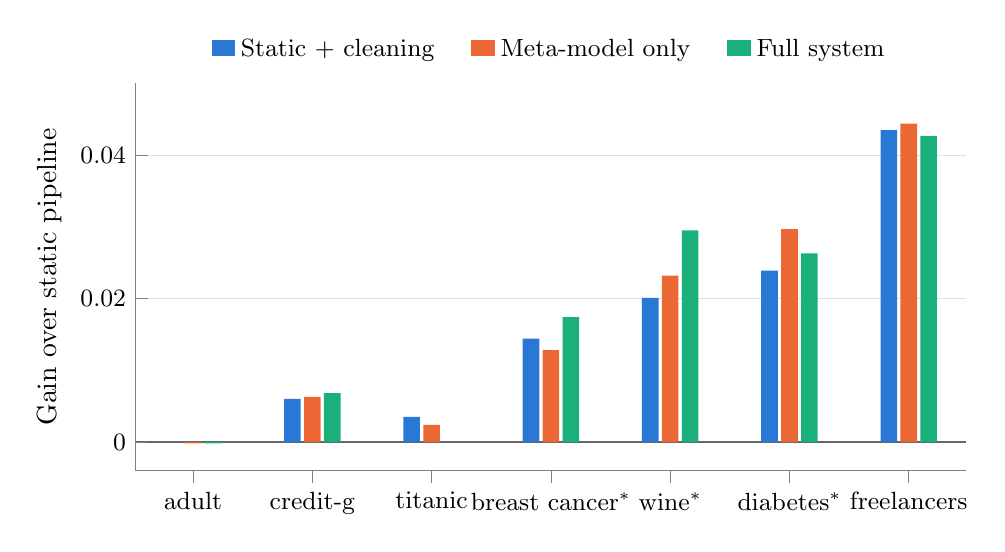
\begin{tikzpicture}
\begin{axis}[
    width=\linewidth,
    height=6.5cm,
    ybar=1.2pt,
    bar width=6pt,
    ymin=-0.004, ymax=0.05,
    scaled y ticks=false,
    ylabel={Gain over static pipeline},
    symbolic x coords={adult, creditg, titanic, breast, wine, diabetes, freelancers},
    xtick=data,
    xticklabels={adult, credit-g, titanic, breast cancer$^\ast$, wine$^\ast$, diabetes$^\ast$, freelancers},
    x tick label style={font=\small},
    y tick label style={font=\small, /pgf/number format/fixed, /pgf/number format/precision=2},
    ymajorgrids,
    major grid style={black!12},
    axis x line*=bottom,
    axis y line*=left,
    axis line style={black!50},
    tick style={black!50},
    enlarge x limits=0.08,
    extra y ticks={0},
    extra y tick labels={},
    extra y tick style={grid=major, major grid style={black!60}},
    legend style={at={(0.5,1.03)}, anchor=south, legend columns=-1, draw=none, font=\small,
                  /tikz/every even column/.append style={column sep=0.4cm}},
    legend image code/.code={\fill[#1] (0cm,-0.08cm) rectangle (0.3cm,0.12cm);},
]
\addplot[fill=cleaning, draw=none] coordinates {
    (adult,0.0000) (creditg,0.0060) (titanic,0.0035) (breast,0.0144) (wine,0.0201) (diabetes,0.0239) (freelancers,0.0435)};
\addplot[fill=metaonly, draw=none] coordinates {
    (adult,-0.0002) (creditg,0.0063) (titanic,0.0024) (breast,0.0128) (wine,0.0232) (diabetes,0.0297) (freelancers,0.0444)};
\addplot[fill=fullsystem, draw=none] coordinates {
    (adult,-0.0002) (creditg,0.0068) (titanic,0.0000) (breast,0.0174) (wine,0.0295) (diabetes,0.0263) (freelancers,0.0427)};
\legend{Static + cleaning, Meta-model only, Full system}
\end{axis}
\end{tikzpicture}
\caption{Mean gain in downstream score over the static pipeline (macro F1 or $R^2$; values in Table~\ref{tab:results}). Real OpenML datasets on the left, datasets with defects on the right ($^\ast$ = injected, freelancers = messy as delivered). The gain appears wherever values need cleaning, and the three configurations that clean are close together.}
\label{fig:gain}
\end{figure}

Value cleaning also keeps the feature space compact. Because the static pipeline one-hot encodes identifiers and free text, it produces 198 to 1,543 features on the datasets that contain them, against 11 to 50 for the full system. On Titanic, static + cleaning still produces 888 features, because forced one-hot encoding expands the high-cardinality ticket, cabin and home destination columns, while the meta-learner's choice of label encoding keeps 11.

\subsection{Ablation Study}

Because every configuration is scored on the identical split, each dataset and split forms one paired comparison, giving 35 pairs per comparison (Table~\ref{tab:ablation}).

\begin{table}[ht]
\centering
\caption{Paired comparisons over 7 datasets $\times$ 5 splits (score averaged over both downstream models).}
\label{tab:ablation}
\begin{tabular}{lcccc}
\toprule
\textbf{Comparison} & \textbf{Wins} & \textbf{Ties} & \textbf{Losses} & \textbf{Mean difference} \\
\midrule
Static + cleaning vs.\ static & 24 & 5 & 6 & +0.0159 \\
Full system vs.\ static + cleaning & 18 & 5 & 12 & +0.0016 \\
Full system vs.\ meta-model only & 10 & 17 & 8 & +0.0006 \\
Full system vs.\ static & 28 & 0 & 7 & +0.0175 \\
\bottomrule
\end{tabular}
\end{table}

Value cleaning accounts for about 90\% of the total gain (0.0159 of 0.0175). Testing strategies against the target wins slightly more often than it loses against good fixed defaults, but the mean difference of 0.0016 is an order of magnitude smaller than the variation between splits (standard deviations of 0.007 to 0.054). Compared with the predicted strategy alone, the full system produces identical scores in 17 of 35 cases, in which evaluation confirmed the prediction, and otherwise wins and loses about equally often. The downstream models do not always agree either: on Titanic, the linear model scores the full system lower than the static pipeline (0.771 against 0.781), while the random forest scores it higher (0.783 against 0.773).

\subsection{Meta-Model Accuracy}

To test whether meta-features predict the best strategy, meta-models were trained on 150 synthetic datasets per task and evaluated with 5-fold cross-validation (Table~\ref{tab:metamodel}). Top-1 counts how often the best strategy is ranked first; top-2 counts how often it is among the two candidates that the Top-K step evaluates.

\begin{table}[ht]
\centering
\caption{Share of synthetic datasets for which the best strategy is found (150 per task, cross-validated).}
\label{tab:metamodel}
\setlength{\tabcolsep}{4pt}
\begin{tabular}{lccccc}
\toprule
\textbf{Task} & \textbf{Majority guess} & \textbf{Rules top-1} & \textbf{Model top-1} & \textbf{Rules top-2} & \textbf{Model top-2} \\
\midrule
Imputation & 0.44 & 0.25 & 0.46 & 0.57 & \textbf{0.73} \\
Scaling & 0.69 & 0.65 & 0.67 & 0.80 & \textbf{0.84} \\
Encoding & 0.69 & 0.41 & 0.66 & 1.00 & 1.00 \\
\bottomrule
\end{tabular}
\end{table}

As a single prediction, the trained meta-model barely beats always guessing the most common strategy for imputation (0.46 against 0.44) and falls slightly short of it for scaling and encoding. The fixed rules are weaker still, particularly for imputation (0.25). As a shortlist the meta-model is more useful: the best imputation strategy is among its two candidates in 73\% of cases, against 57\% for the rules. For encoding, top-2 is trivially 1.00 because there are only two strategies. A benchmark run with these trained meta-models did not improve downstream results (mean rank of the full system 2.29, against 2.21 with the fixed rules).

\subsection{Comparative Advantages of the Proposed Framework}

The architecture of the proposed system offers several distinct advantages over traditional automated preprocessing pipelines:
\begin{itemize}
    \item \textbf{Repairing values before modelling.} Standardising yes/no text, numbers stored as text and spelling variants is the component with the largest measured effect, and it requires no expert configuration.
    \item \textbf{Leakage-safe evaluation.} The target never passes through feature preprocessing, and in the benchmark strategies are chosen on rows other than those they are scored on.
    \item \textbf{Adaptive data retention vs.\ lossy deletion.} Standard preprocessing workflows often handle outliers by removing the affected rows, which can bias the dataset and reduce statistical power. By utilizing IQR-based Winsorization, the system preserves the total sample size while neutralizing the influence of extreme noise, and the human-readable output keeps the original values.
    \item \textbf{Compact feature space.} Excluding identifiers and using label encoding for columns with many categories keeps 11 to 90 features where a static pipeline creates up to 1,543.
    \item \textbf{Auditability and transparency.} The system generates a comprehensive JSON audit trail via the DecisionLogger, recording the before/after state of every transformed column, the candidate scores and the rationale for each decision.
\end{itemize}


\section{Discussion}

The results support automating data preparation, but they locate the benefit differently than expected. The measurable improvement over a static pipeline comes from repairing values and excluding identifiers, not from choosing between imputation and scaling strategies. On these datasets, the candidate strategies usually score within the noise of one another, so selecting the best one adds little over a sensible default. This is consistent with the meta-model results: if strategies rarely differ much, the statistics of a single column have little to predict, and neither the fixed rules nor the trained meta-model identifies the best strategy reliably. Evaluation against the target remains useful as a safeguard, because it measures rather than assumes, and its cost is small (about 0.2\,s more per run in the benchmark).

These findings have limitations. The benchmark covers seven datasets, and the defects in three of them were injected synthetically; they were designed to resemble real exports but correspond to what the cleaning step repairs, which favours the cleaning configurations. The meta-features describe only one column per decision, and the meta-models were trained on synthetic data only. Absolute scores are slightly optimistic, as described in the experimental setup.

In addition, the system prioritizes local optimization rather than global pipeline search. While this reduces computational complexity, it may miss interactions between preprocessing stages. For example, the optimal encoding strategy may depend on the chosen scaling method. Addressing such dependencies remains an open challenge.

Another limitation concerns computational cost on large datasets. Although mitigation strategies are employed, fully automated evaluation-based preprocessing may not be suitable for real-time or resource-constrained environments. Hybrid approaches combining meta-learning with offline knowledge bases may offer a promising solution.


% ---------------- OPEN QUESTIONS ----------------
\section{Open Questions and Future Work}

The proposed system performs local optimization at each preprocessing stage rather than global pipeline optimization, and its strategy selection adds little on the datasets studied. Future research directions include:

\begin{itemize}
    \item Joint optimization of preprocessing pipelines
    \item Meta-features that describe the whole dataset and the relationship between columns and target, rather than a single column
    \item Meta-training on real datasets in addition to synthetic ones
    \item A larger benchmark of real, messy datasets, so that cleaning can be evaluated without injected defects
    \item Reinforcement learning for strategy selection
    \item Extension to non-tabular and multimodal data
\end{itemize}

Additionally, computational efficiency remains a challenge when evaluating multiple candidate strategies on large datasets.

% ---------------- LITERATURE ----------------
\section{Literature}

This paper intentionally omits formal literature citations in accordance with the assignment requirements. Nevertheless, the proposed framework builds upon established concepts in meta-learning, automated machine learning, and performance-driven optimization.


\begin{thebibliography}{99}

\bibitem{kuhn2019feature}
M. Kuhn and K. Johnson,
\textit{Feature Engineering and Selection: A Practical Approach for Predictive Models},
CRC Press, 2019.

\bibitem{garcia2015data}
S. Garcia, J. Luengo, and F. Herrera,
\textit{Data Preprocessing in Data Mining},
Springer, 2015.

\bibitem{bilalli2017automated}
B. Bilalli, A. Abelló, and T. Aluja-Banet,
``Automated data preprocessing for Big Data,''
\textit{Proceedings of the International Conference on Big Data Analytics}, 2017.

\bibitem{he2019automl}
X. He, K. Zhao, and X. Chu,
``AutoML: A survey of the state-of-the-art,''
\textit{Knowledge-Based Systems}, vol. 212, 2021.

\bibitem{vanschoren2019metalearning}
J. Vanschoren,
``Meta-learning: A survey,''
\textit{Foundations and Trends in Machine Learning},
vol. 11, no. 1, pp. 1--224, 2019.

\bibitem{feurer2015efficient}
M. Feurer et al.,
``Efficient and robust automated machine learning,''
\textit{Advances in Neural Information Processing Systems (NeurIPS)}, 2015.

\bibitem{zoller2021survey}
M.-A. Zöller and M. F. Huber,
``Benchmark and survey of automated machine learning frameworks,''
\textit{Journal of Artificial Intelligence Research}, vol. 70, pp. 409--472, 2021.

\bibitem{bergstra2012random}
J. Bergstra and Y. Bengio,
``Random search for hyper-parameter optimization,''
\textit{Journal of Machine Learning Research}, vol. 13, pp. 281--305, 2012.

\bibitem{guyon2006feature}
I. Guyon and A. Elisseeff,
``An introduction to variable and feature selection,''
\textit{Journal of Machine Learning Research}, vol. 3, pp. 1157--1182, 2003.

\bibitem{domingos2012few}
P. Domingos,
``A few useful things to know about machine learning,''
\textit{Communications of the ACM}, vol. 55, no. 10, pp. 78--87, 2012.

\end{thebibliography}


\end{document}
